%!TEX root=./report.tex
\section{ARCHITECTURE AND IMPLEMENTATION}
Our evaluation framework is built around classes from PCL~\cite{PCL} and VTK~\cite{vtk}.
The stock detection algorithm relies heavily PCL, which does all of the lower level work.
We use the Princeton Shape Benchmark.
Since the dataset contains polygonal representations, the framework uses simulated lidar scanning to create point clouds. We use SyntheticLidarScanner~\cite{Doria2009}, which provides a feature-rich utility which allows us to control the point cloud resolution and noisiness.

Our evaluation framework has two major parts. First is the Detector class, which houses the detection logic. Second is the Proctor class, which generates tests and reports. These are illustrated in \autoref{fig:arch}.

\begin{figure}[thpb]
  \centering
  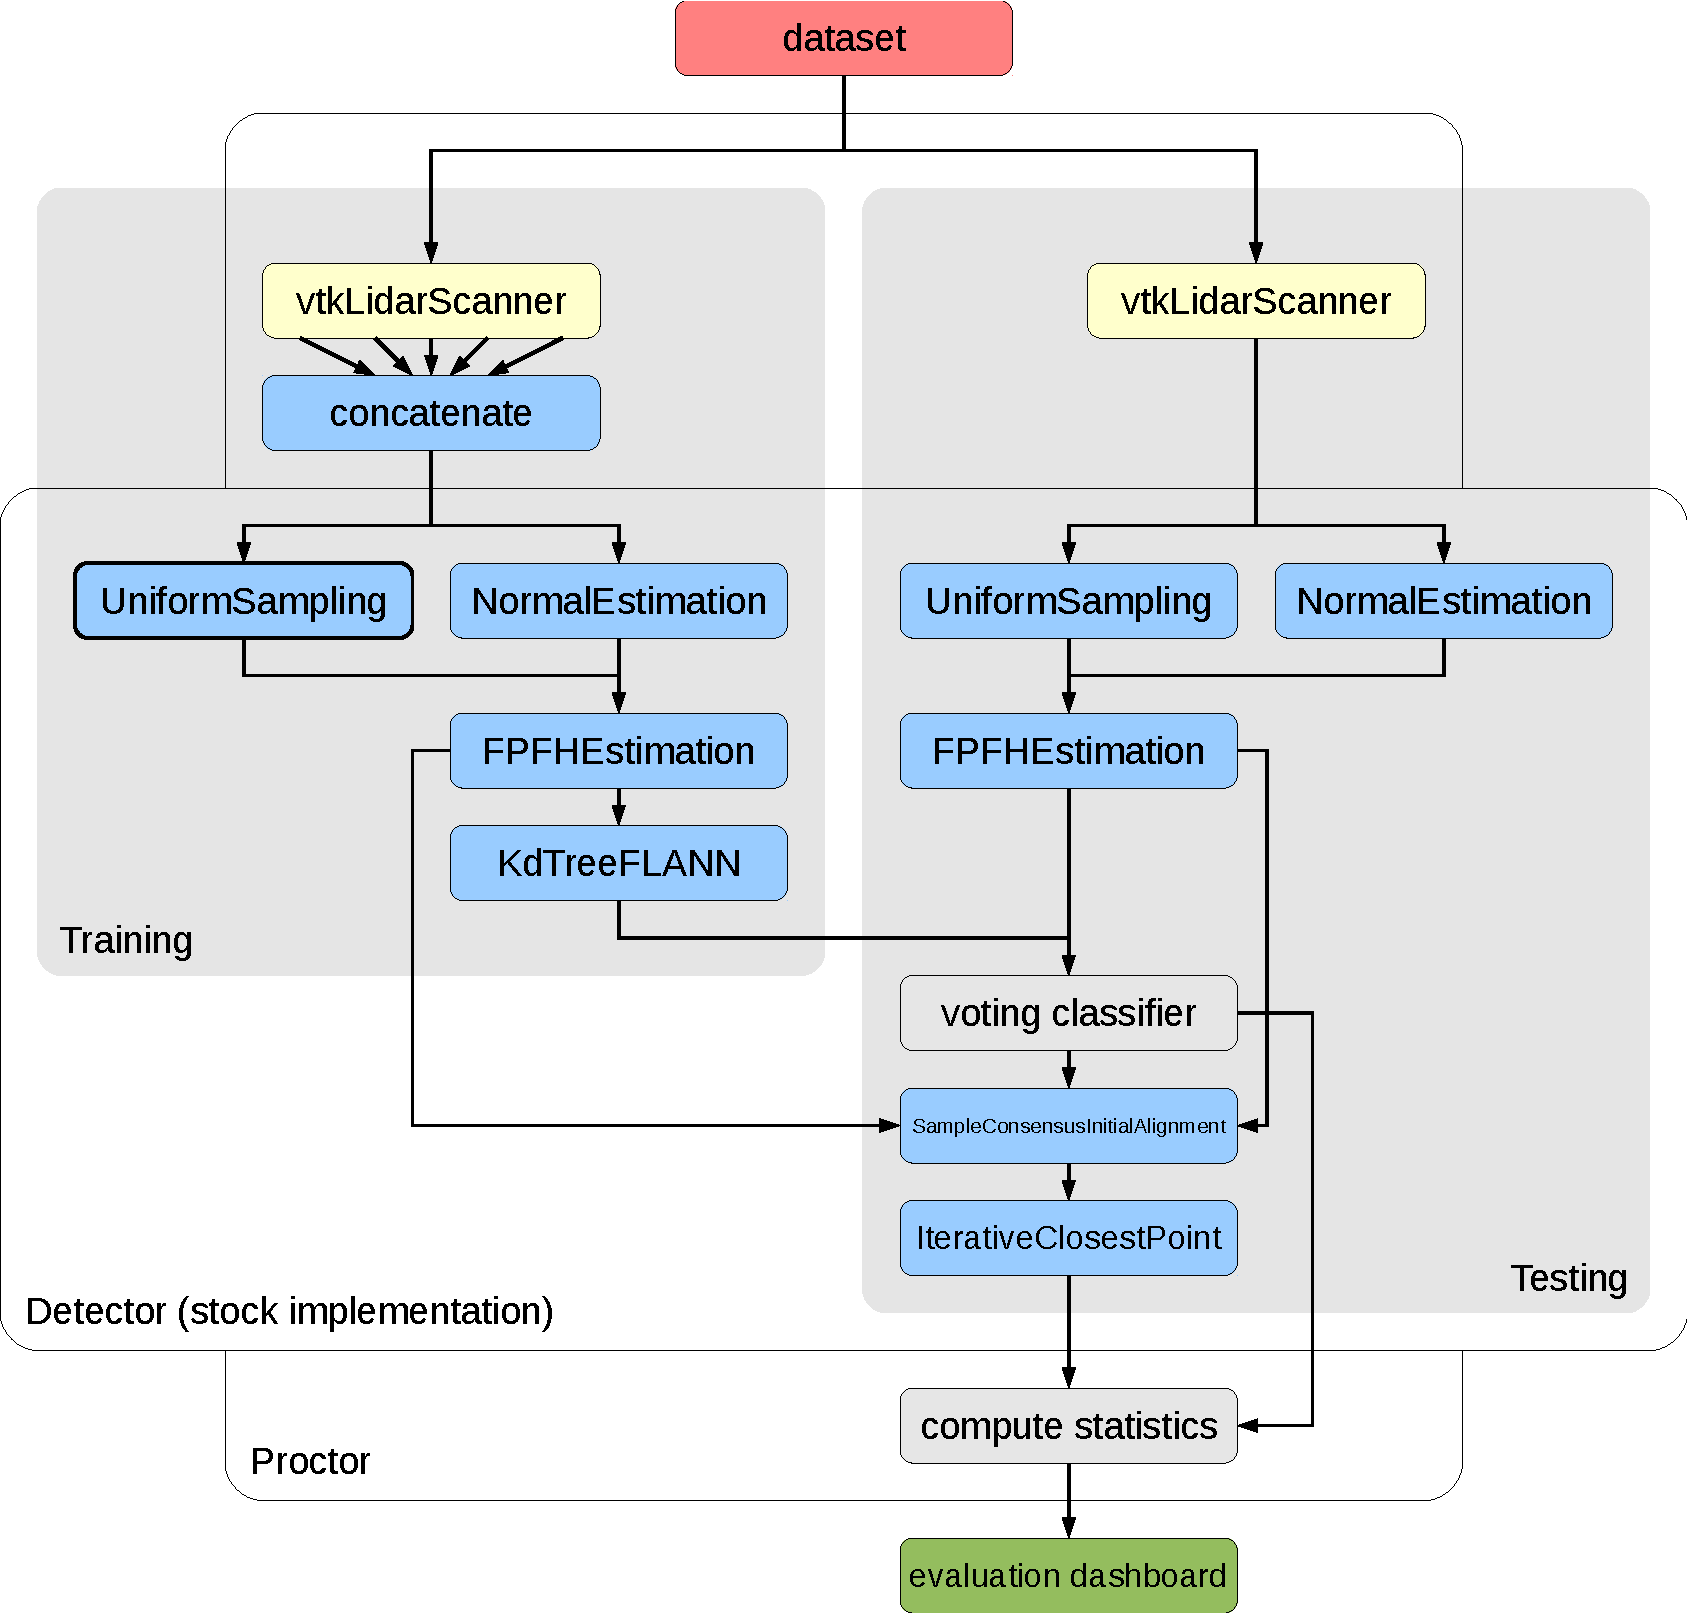
\includegraphics[width=\columnwidth]{../figures/architecture.pdf}
  \caption{Architectural overview of Proctor and stock Detector implementation}
  \label{fig:arch}
\end{figure}

\subsection{Detector}
In designing this class, we tried to accommodate a common strategy in detection systems.
These systems typically start by computing a feature on the reference models and placing them in a lookup structure.
Then, a classification algorithm use this structure to narrow down the candidate models to a few likely fits.
Finally, it attempts to register the query scene with the likely candidates. This is usually more expensive than the feature computation and classification.

A custom detector must follow an interface with methods that take training data and test queries.
For training, the detector receives the full point cloud of each model.
For testing, the detector receives a range scan of some model, at some angle. It must output an estimated similarity for each candidate model, a more precise estimated distance to some candidate models, and a best guess of which model was scanned.
In particular, we intend that detection systems that fit the description in the previous paragraph populate the similarities with classifier scores and populate the precise distances with Euclidean distances after registration.
Ultimately, the Detector class is intended to be something that algorithm authors shall edit.

\subsubsection{Primary Stock Detector}
We are publishing the current contribution with a few stock detectors, which serve as both a scaffolding for modular enhancements and baselines for larger efforts.
The primary stock implementation makes use of Fast Point Feature Histograms~\cite{fpfh1, fpfh2}, a voting-based classification algorithm, and registration.

During training, the stock implementation divides the points of each model into uniform voxels. For each voxel, it picks a representative point that is closest to the centroid of the voxel. This subset is a dense keypoint sampling of the model. It computes the FPFH centered at each of the keypoints. A KdTree is built from these feature histograms and stored for later use.

During testing, the stock implementation starts the same way as training: it uses a voxel grid to generate a dense keypoint set, and computes FPFH on those keypoints.
For each keypoint in the query scene, the implementation searches the KdTree built during training for the four nearest neighbors in feature space. Each of these results contributes a vote for the corresponding model, weighted by the reciprocal of the $L^2$ distance between the scene feature vector and the model feature vector.
The implementation then tries to register the query with the four candidate models that have the greatest total votes.
This is done by first using the initial alignment algorithm described in section IV of the FPFH paper, then, running a few iterations of ICP.
A screenshot of the visualization provided by the stock detector is provided in \autoref{fig:vis}.
\begin{figure}[thpb]
  \centering
  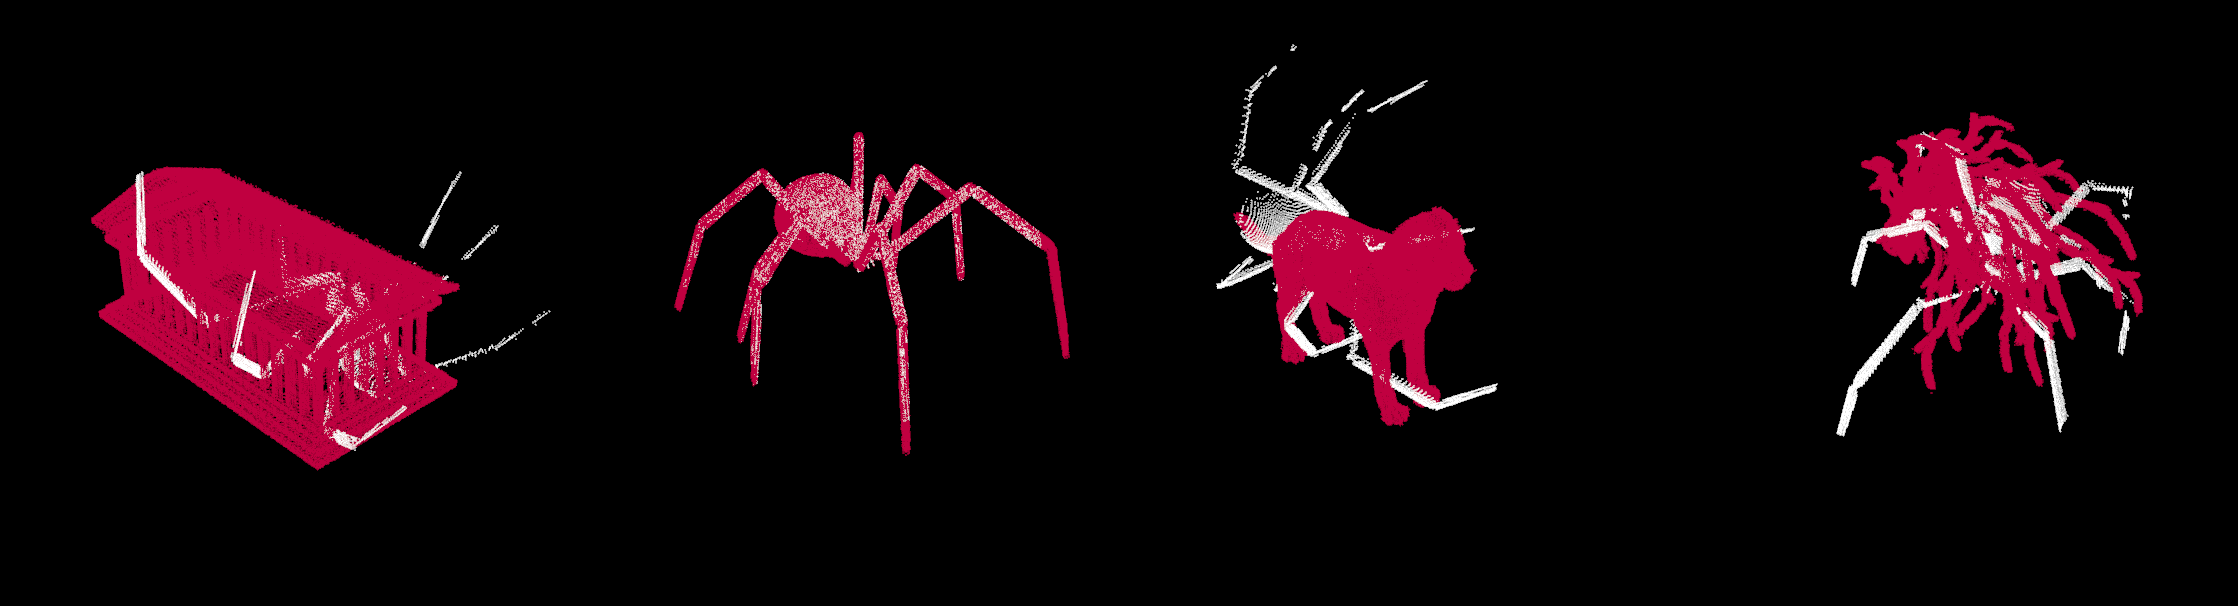
\includegraphics[width=\columnwidth]{../figures/visualization.png}
  \caption{Visualization of registration results in a particular test trial}
  \label{fig:vis}
\end{figure}

The vote totals are output as the estimated likeness ratings.
The registered distance from the four top canidates are returned as the estimated euclidean distances.
Finally, the model that registers most closely with the scene is selected as the detected model.

\subsubsection{Stock Variants}
Other detectors already in place are variants that replace FPFH with other local features supported by PCL. There are branches using PFH~\cite{pfh1, pfh2}, spin images~\cite{SpinImages}, and SHOT~\cite{shot}.
The classification and registration mechanisms remain the same.

\subsection{Proctor}
The Proctor class surrounds calls to the Detector's interface with logic for capturing synthetic range scans as well as code for compiling raw results into popular statistics.
The evaluation program takes up to two arguments, used as random number generator seeds.

The first seed is used to select a random subset of models from the dataset. If omitted, the default seed is a constant value.
The selected models are read from disk, along with some of the metadata included in the dataset.
From the loaded polygonal models, the program generates the full point clouds for testing by running a virtual range scan from uniform angles around the model's center of mass.
The virtual scanner's distance is computed as a constant times the average distance from all points on the surfaces of all polygons to the center of mass.
The program then passes the full point clouds to the Detector for training.

The second seed is used to generate a series of test vectors, which consist of a random model and a random angle.
For each test vector, the program runs a virtual range scan of the selected model from the selected angle.
The program then passes the range scan to the Detector for training.

After all test trials have completed, the program uses the output from the Detector to compute the metrics described in the next section.
